\documentclass[border=0pt]{standalone}
\usepackage[T1]{fontenc}
\usepackage{lmodern}

\usepackage{tikz}
\usetikzlibrary{calc}
\begin{document}%
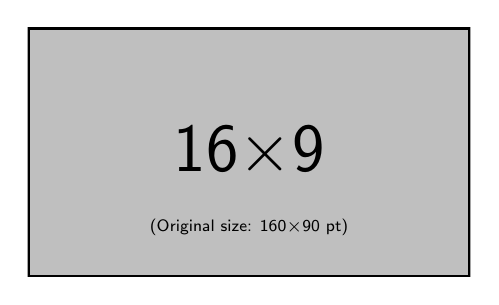
\begin{tikzpicture}[x=16pt,y=9pt]%
    \clip (0,0) rectangle (10,10);
    \path [draw,fill=black!25,ultra thick] (0,0) rectangle (10,10);
    \path let \p1=(2,0), \p2=(2.4,0), \p3=(.4,0), \p4 = (.48,0) in
       node at (5,5) {\sffamily\fontsize{\x1}{\x2}\selectfont 16$\times$9}
       node at (5,2) {\sffamily\fontsize{\x3}{\x4}\selectfont (Original size: 160$\times$90 pt)}
    ;
\end{tikzpicture}%
\end{document}%
